%% It is just an empty TeX file.
%% Write your code here.
\graphicspath{{sec04/images/}{sec04/code/}}
\lstset{inputpath=sec04/code/}

\begin{frame}{Entities}

\begin{enumerate}
    \item Primitive commands
    \item Macros
    \item Counters (=integer numbers)
    \item Lengths
    \item Glues
    \item Boxes
    \item Strings
\end{enumerate}
\incPause
We already see something about all this stuff except counters. Let us look at them! (And then return to look deeper at the boxes, lengths, glues and strings)
     
\end{frame}

\subsection{Counters}
\begin{frame}{What is ``counter''}\relax

``Counter'' is just an integer number.

It's using in multiple places to count everything in \LaTeX: sections, equations, references, citation, enumerate lists,...
     
\end{frame}

\begin{frame}{Define and simple manipulation with counters \lW}\relax
\twocolImg{
\lstinputlisting[linerange={11-18}]{countersimp.tex}
}{countersimp}

\begin{itemize}
    \item \ccol\newcounter\ to define new counter 
    \item \ccol\setcounter\ to set counter to new value
    \item \ccol\addtocounter\ to add a number to the counter
\end{itemize}

\skfootnote{\lvoc{VII.3.1}[244] \lmanc{12.5}[117] \lmanc{13.4-5}[128] \wikiC{https://en.wikibooks.org/wiki/LaTeX/Counters\#Counter_manipulation}}
     
\end{frame}

\inclassFrame{

\begin{frame}{Try it out}\relax

     \lstinputlisting{countersimpTASK.tex}

\end{frame}}

\begin{frame}{Print counter\lW}\relax
     
     \newcommand{\countab}[1]{\newcounter{tmptt}
     \ccol#1\{countname\}&
     \setcounter{tmptt}{1} #1{tmptt} &
     \setcounter{tmptt}{2} #1{tmptt} &
     \setcounter{tmptt}{3} #1{tmptt} &
     \setcounter{tmptt}{4} #1{tmptt} &
     \setcounter{tmptt}{5} #1{tmptt} &
     \setcounter{tmptt}{6} #1{tmptt} &
     \setcounter{tmptt}{7} #1{tmptt} &
     \setcounter{tmptt}{8} #1{tmptt} &
     \setcounter{tmptt}{9} #1{tmptt}
     \\}
     
     \begin{tabular}{l|ccccccccc}
          \countab{\arabic}
          \countab{\alph}
          \countab{\Alph}
          \countab{\roman}
          \countab{\Roman}
          \countab{\fnsymbol}
     \end{tabular}
     \vspace{1ex}
     
     P.S. \ccol\value\ to get ``raw'' value of the counter
     \skfootnote{ \wikiC{\https://en.wikibooks.org/wiki/LaTeX/Counters\#Counter_style} \lmac{13.1}[126]\\ 
     see \lvoc{IX.2.3}[295] for russian analog of \ccol\alph}
\end{frame}

\begin{frame}{pre-defined counters in standart classes}
\newlength{\myboxlen}%
\setlength{\myboxlen}{5em}

\newcommand{\showC}[1]{%
\makebox[\myboxlen]{#1\hfill}%
}

\showC{part}\hfill
\showC{chapter}\hfill
\showC{section}\hfill
\showC{subsection}\hfill
\showC{subsubsection}\hfill
\showC{paragraph}\hfill
\showC{subparagraph}\hfill
\showC{}\hfill
\showC{}\hfill
\showC{}\hfill
\showC{}\hfill
\showC{}\hfill

\showC{page}\hfill
\showC{figure}\hfill
\showC{table}\hfill
\showC{footnote}\hfill
\showC{equation}\hfill

\showC{enumi}\hfill
\showC{enumii}\hfill
\showC{enumiii}\hfill
\showC{enumiv}\hfill
\showC{}\hfill
\showC{}\hfill
\showC{}\hfill
\showC{}\hfill
\showC{}\hfill

\TeX's counters (will talk later)
\showC{\ccol\year}\hfill
\showC{\ccol\month}\hfill
\showC{\ccol\day}\hfill
\showC{\ccol\time}\hfill
\showC{}\hfill
\showC{}\hfill
\showC{}\hfill
\showC{}\hfill
\showC{}\hfill



\skfootnote{\wikiC{https://en.wikibooks.org/wiki/LaTeX/Counters\#LaTeX_default_counters} \lmanc{13}[126]}
\end{frame}

\begin{frame}{Counter Domination\inClass{, conquering, humiliation}}{problem}\relax
\begin{columns}
\begin{column}{0.45\textwidth}
     You may want to write something like
     
     \vspace{-5ex}
     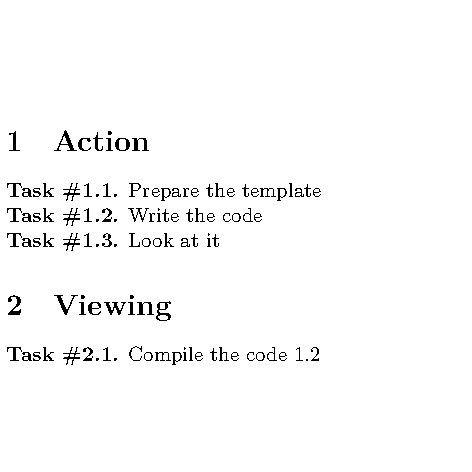
\includegraphics[width=\linewidth]{counterdom}
\end{column}
\incPause
\begin{column}{0.45\textwidth}
But the straightforward solution will give you 

\vspace{-5ex}
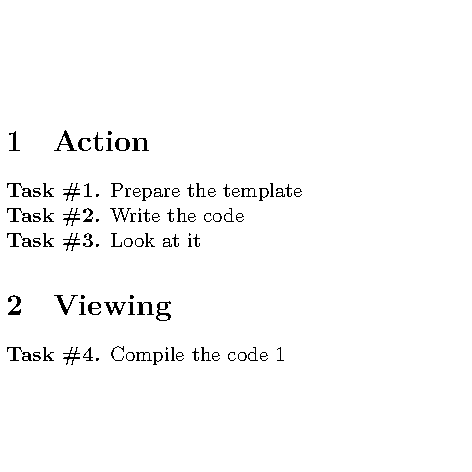
\includegraphics[width=\linewidth]{counterdomno}
     
\end{column}
     
\end{columns}
\end{frame}

\begin{frame}{Counter Domination\inClass{, conquering, humiliation}}{straightforward solution}\relax

\twocolImg{
\lstinputlisting[linerange={11-20}]{counterdomno.tex}
}{counterdomno}

\inclassFrag{Modify your code so it will look the same way}[0]
\end{frame}

\begin{frame}[fragile]{Counter Domination\inClass{, conquering, humiliation}}{The Way}\relax

\newcommand{\modif}[3]{\fbox{\parbox{\textwidth}{\makebox[\textwidth]{\small\makebox[0.47\textwidth]{#1}\hfill$\to$\hfill\makebox[0.47\textwidth]{#2}}\\ #3}}}

\centering
\modif{\string\newcounter\{task\}}{\ocol\newcounter\{task\}[section]}{\ocol\newcounter\{<slave>\}[<master>] will resets the value of <slave> if the value of <master> is change}

\inclassFrag{Please, modify your code after this and every step in this frame}
% \incPause

\modif{\ccol\addtocounter\{task\}\{1\}}{\ccol\refstepcounter\{task\}}{
\ccol\refstepcounter\{<counter>\} use it to update \ccol\label--\ccol\ref\ mechanism
}

\incPause
\modif{\string\textbf\{Task \string\#\string\arabic\{task\}.}{\tiny\string\textbf\{Task \string\#\string\arabic\{section\}.\string\arabic\{task\}.}{Inside \string\newcommand\{\string\tsk\} to redefine the labels}

\incPause
\modif{}{\tiny\string\renewcommand\{\ccol\thetask\}\{\string\arabic\{section\}.\string\arabic\{task\}\}}{\string\renewcommand\{\ccol{\the<counter>}\} to redefine the reference}

\skfootnote{\lvoc{VII.3.3}[250] \lmanc{13.6}[128]}
\end{frame}


\begin{frame}{Counter Domination\inClass{, conquering, humiliation}}{solution}\relax
\twocolImg{
\lstinputlisting[linerange={11-20}]{counterdom.tex}
}{counterdom}
\end{frame}

\begin{frame}[fragile]{Redefine existing counter domination\magicPage}{``equation'' example}\relax
Package based solution:

\lstinline|\usepackage{chngcntr}| 

and \lstinline|\counterwith{equation}{chapter}|  to make the ``equation'' a slave or \lstinline|\counterwithout{equation}{chapter}| to ``free'' the counter.

Core-based solution:

\begin{lstlisting}
\makeatletter
\@removefromreset{equation}{section}
\@addtoreset{equation}{chapter}
\renewcommand{\theequation}{\thechapter.\@arabic\c@equation}
\makeatother
\end{lstlisting}


\skfootnote{\vspace{-10ex}\stExC{https://tex.stackexchange.com/questions/61756/how-to-change-equation-numbering-style} \stExC{https://tex.stackexchange.com/questions/54241/change-the-type-of-equation-numbering-in-document-class-article} \stExC{https://tex.stackexchange.com/questions/28333/continuous-v-per-chapter-section-numbering-of-figures-tables-and-other-docume} \normalfont\url{https://texfaq.org/FAQ-running-nos} \lvoc{IX.2.1}[293].\\ Also see \ccol{\p@} prefix \lvoc{IX.2.2}[295] and \stExC{https://tex.stackexchange.com/questions/61426/how-to-make-ref-display-only-subsection}}     
\end{frame}


\begin{frame}[fragile]{Define and simple manipulation\tW\magicPage}\relax

     \textbf{Define new} \ccol\newcount\ccol{\<countname>} as \verb|\newcount\mycounter|
     
     \textbf{Set number} \ccol{\<countname>=<number>}  Or use \ccol\countdef. Like \verb|\countdef\mynumber=43|
     
     \textbf{Add number}  \ccol{\advance\string\<countname>\ by <number>}. Also there are \ccol\multiply\ and \ccol\divide. As well as \ccol\numexp.
     
     \textbf{Show number} \ccol{\the\string\<countname>} or \ccol\number\ or \ccol\romannumeral
     
     \skfootnote{\vspace{-3ex}\knuthc{15}[129] \stExC{https://tex.stackexchange.com/questions/245635/formal-syntax-rules-of-dimexpr-numexpr-glueexpr}\\Actually you can use \ccol\count<number> like \ccol\count212. What \ccol\newcount\ do is just find a free number and fix it to your defined name.}
\end{frame}

\begin{frame}{Define and simple manipulation\tW\magicPage}{Example}\relax

\twocolImg{
\lstinputlisting[linerange={11-16}]{counterTeX.tex}
}{counterTeX}

\end{frame}

\subsection{Length}


\begin{frame}{Length manipulation\tW\magicPage}\relax

\textbf{Define lenght} \ccol{\newdimen\string\<lenname>}

\textbf{Set length} \ccol{\string\<lenname>=<len>}

\textbf{Add lenght}  \ccol{\advance\string\<lenname>\ by <len>}. Also there are \ccol\multiply\ and \ccol\divide. As well as \ccol\dimexp.

\textbf{Show lenght} \ccol{\the\string\<lenname>}


\skfootnote{\knuthc{15}[132] }
\end{frame}

\begin{frame}{Length manipulation\tW\magicPage}{Example}\relax

\twocolImg{
\lstinputlisting[linerange={11-14}]{lengthTeX.tex}
}{lengthTeX}

\end{frame}


\begin{frame}{Length manipulation\lW\magicPage}\relax

\textbf{Define lenght} \ccol{\newlength\{\string\<lenname>\}}

\textbf{Set length} \ccol{\setlength}

\textbf{Add lenght}  \ccol{\addtolength}. 

\textbf{Show lenght} \ccol{\the\string\<lenname>}. But also you can use \ncol\usepackage{printlen}\ and then \ccol\uselengthunit, \ccol\printlength



\skfootnote{\wikiC{https://en.wikibooks.org/wiki/LaTeX/Lengths} }
\end{frame}

\begin{frame}{Length manipulation\lW\magicPage}{Example}\relax

\twocolImg{
\lstinputlisting[linerange={7-7,11-16}]{lengthLaTeX.tex}
}{lengthLaTeX}

\end{frame}

\subsection{Skips}

\begin{frame}{Skip manipulation\tW\magicPage}\relax

\TeX\ provides additional storage for glue and glue in math mode (that is sensible for math style). They have the same syntax as length, just with \ccol\skip\ or \ccol\muskip\ prefix/suffix
\end{frame}

\subsection{Toks}

\begin{frame}{Toks manipulation\tw\magicPage}\relax

\TeX\ has addition registers for storing strings. They have \ccol\toks\ prefix/suffix. The difference between toks and storage inside macros are in extension... 
     
     \skfootnote{\stExC{https://tex.stackexchange.com/questions/455208/token-register-vs-macro-register}}
\end{frame}


\subsection{Boxes}

\begin{frame}{Box manipulation\tW\magicPage}\relax

\textbf{Define box} \ccol{\newbox\string\<boxname>}

\textbf{Set box} \ccol{\setbox\string\<boxname>=<box>}

\textbf{Provide the content without deleting it:} \ccol{\copy\string\<boxname>}

\textbf{Provide the content with delete from memory:} \ccol{\box\string\<boxname>}

\textbf{Dimentions}: width: \ccol\wd, height: \ccol\ht, depth: \ccol\dp

\skfootnote{\knuthc{15}[131] }
\end{frame}

\begin{frame}{Box manipulation\tW\magicPage}{Example}\relax

\twocolImg{
\lstinputlisting[linerange={12-20}]{boxTeX.tex}
}{boxTeX}

\skfootnote{\ccol\the\ here is just to PRINT the length. Not the part of the command.}
\end{frame}


\begin{frame}[fragile]{Box manipulation\lW\magicPage}\relax

\textbf{Define box} \ccol{\newsavebox\{\string\<boxname>\}}

\textbf{Set box} \ccol{\savebox}

\textbf{Provide the content without deleting it:} \ccol{\usebox}

\textbf{Dimentions}: 
\begin{enumerate}
    \item Create a length variable: \ccol\newlength
    \item Set the variable to dimention of the box CONTENT:
    \begin{itemize}
        \item width: \verb|\settowidth{\<len-var>}{\usebox{\<box>}}|
        \item height: \verb|\settoheight{\<len-var>}{\usebox{\<box>}}|
        \item depth: \verb|\settodepth{\<len-var>}{\usebox{\<box>}}|
    \end{itemize}
     
\end{enumerate}

\skfootnote{\lmanc{14.4-6}[133] \lmanc{20.5, 20.7}[183]}
\end{frame}

\begin{frame}{Box manipulation\lW\magicPage}{Example}\relax

\twocolImg{
\lstinputlisting[linerange={12-26}]{boxLaTeX.tex}
}{boxLaTeX}
 
\skfootnote{\ccol\the\ here is just to PRINT the length. Not the part of the command.}
\end{frame}